\section{8.23}
\subsection{b)}
\paragraph{Requirement:}
Calculate the size of the interior angles of the triangle with the given
vertices. \\
$K(0|-3), L(3|5), M(-9|1)$

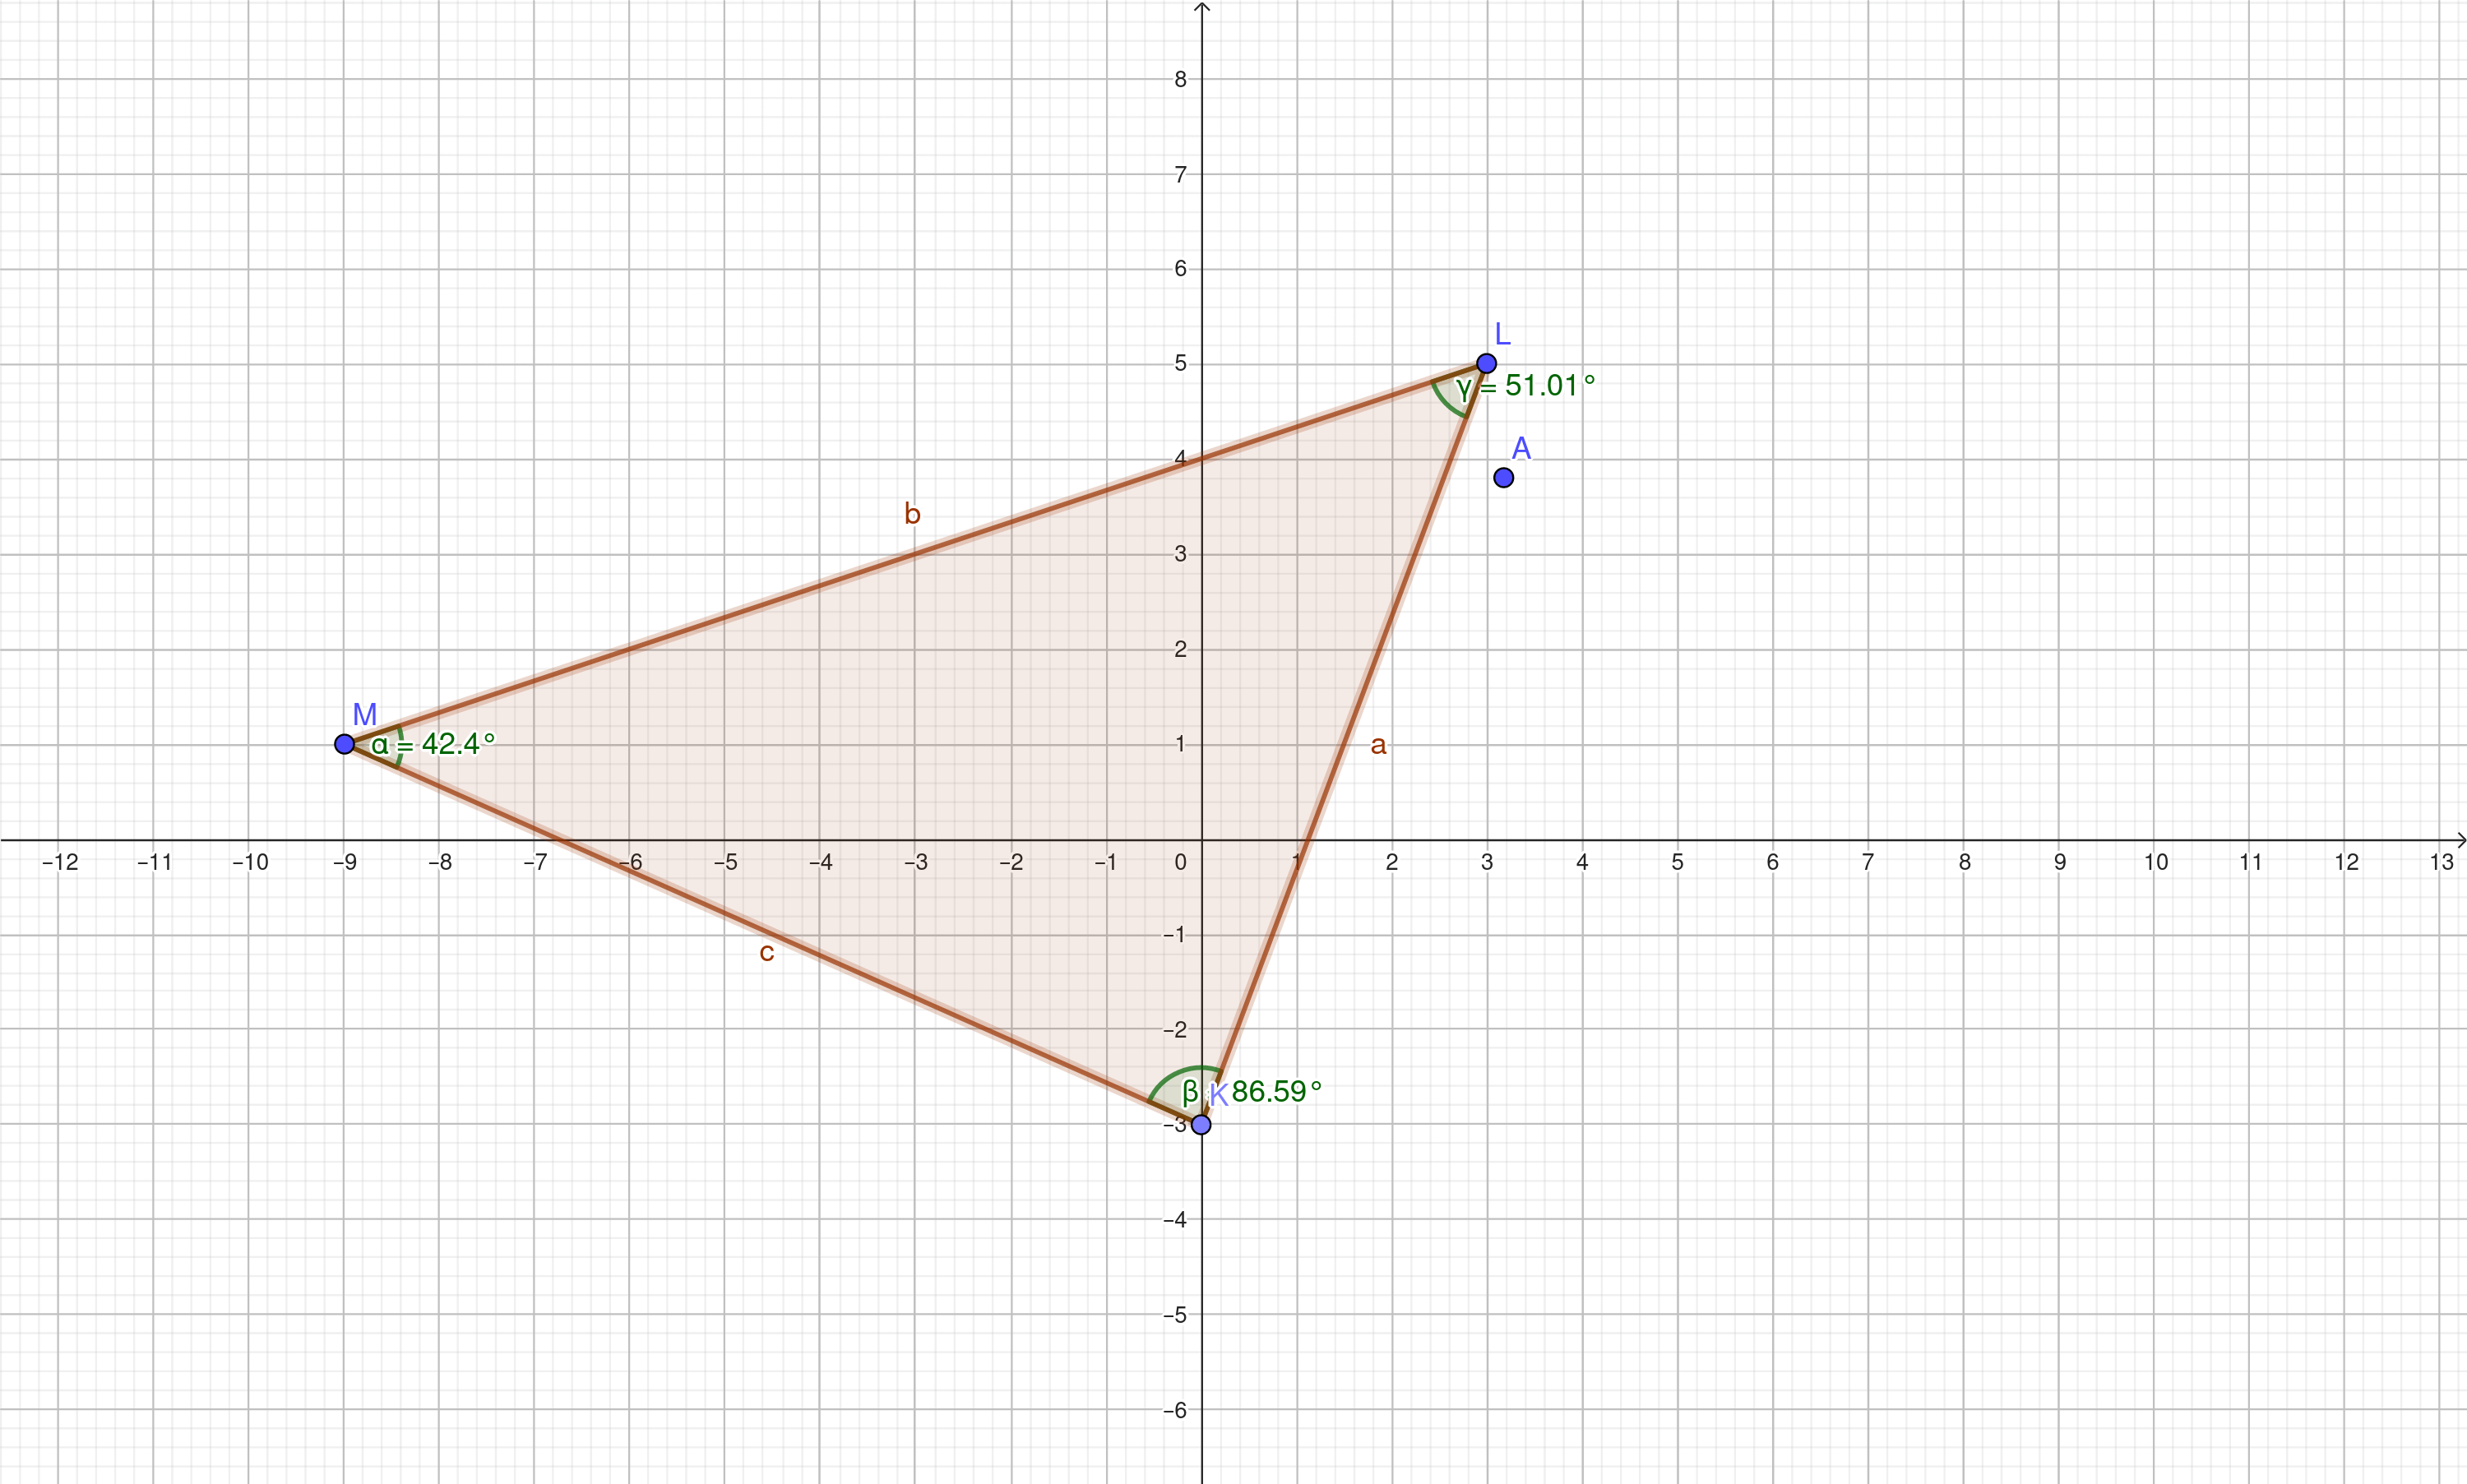
\includegraphics[width=\linewidth]{images/8-23.png}

\def\va{\begin{pmatrix}
   3 \\ 
   8
\end{pmatrix}}
\def\vb{\begin{pmatrix}
   -12 \\ 
   -4
\end{pmatrix}}
\def\vc{\begin{pmatrix}
   9 \\ 
   -4
\end{pmatrix}}

\paragraph{Exercises:}
\begin{align}
   \vec{KL} &= \begin{pmatrix}
       3 \\ 
       5
   \end{pmatrix} - 
   \begin{pmatrix}
       0 \\ 
       -3
   \end{pmatrix} \\
   \vec{KL} &= \va \\[20pt]
   \vec{LM} &= \begin{pmatrix}
       -9 \\ 
       1
   \end{pmatrix} - 
   \begin{pmatrix}
       3 \\ 
       5
   \end{pmatrix} \\
   \vec{LM} &= \vb \\[20pt]
   \vec{MK} &= \begin{pmatrix}
       0 \\ 
       -3
   \end{pmatrix} - 
   \begin{pmatrix}
       -9 \\ 
       1
   \end{pmatrix} \\
   \vec{MK} &= \vc
\end{align}

\begin{align}
    \cos(\alpha) &= \frac{\vec{LM} \cdot (-\vec{MK})}{|\vec{LM}| * |\vec{MK}|} \\
   \cos(\alpha) &= \frac{\vb \cdot (-\vc)}{\sqrt{12^2 + 4^2} * \sqrt{9^2 + 4^2}} \\
   \cos(\alpha) &= \frac{92}{124.579292019} \\
   \alpha &= \arccos(0.738485493929) \\
   \alpha &= 42.39744^\circ \\[20pt]
   \cos(\beta) &= \frac{\vec{KL} \cdot (-\vec{MK})}{|\vec{KL}| * |\vec{MK}|} \\
   \cos(\beta) &= \frac{\va \cdot (-\vc)}{\sqrt{3^2 + 8^2} * \sqrt{9^2 + 4^2}} \\
   \cos(\beta) &= \frac{5}{84.1486779456} \\
   \beta &= \arccos(0.0594186399842) \\
   \beta &= 86.59356^\circ \\[20pt]
   \gamma &= 180^\circ - (\alpha + \beta) \\
   \gamma &= 180^\circ - (42.39744^\circ + 86.59356^\circ) \\
   \gamma &= 51.00901^\circ 
\end{align}
